\documentclass[stu, 11pt, letterpaper, donotrepeattitle, floatsintext, natbib]{apa7}
\usepackage[utf8]{inputenc}
\usepackage{comment}
\usepackage{marvosym}
\usepackage{graphicx}
\usepackage{indentfirst}
\usepackage{float}
\usepackage[normalem]{ulem}
\usepackage[spanish,es-tabla]{babel} 
\usepackage{listings}
\selectlanguage{spanish}
\useunder{\uline}{\ul}{}
\linespread{2}
\usepackage[skip=10pt plus1pt, indent=1.27cm]{parskip}
\setlength{\intextsep}{1cm plus .1cm minus 1.cm}
\usepackage{color}
\usepackage{helvet}
\usepackage{ragged2e}
\usepackage{pdflscape}
\definecolor{dkgreen}{rgb}{0,0.6,0}
\definecolor{gray}{rgb}{0.5,0.5,0.5}
\definecolor{mauve}{rgb}{0.58,0,0.82}
\usepackage{indentfirst}
\lstset{frame=tb,
  language=Java,
  aboveskip=3mm,
  belowskip=3mm,
  showstringspaces=false,
  columns=flexible,
  basicstyle={\small\ttfamily},
  numbers=none,
  numberstyle=\tiny\color{gray},
  keywordstyle=\color{blue},
  commentstyle=\color{dkgreen},
  stringstyle=\color{mauve},
  breaklines=true,
  breakatwhitespace=true,
  tabsize=3
}

\setlength{\parindent}{1.5cm}

% Portada
\thispagestyle{empty}
\title{\Large  TRABAJO DE INVESTIGACIÓN \\ OFICIAL DE PROTECCIÓN DE DATOS}
\author{Gustavo Landaeta Baeza } % (autores separados, consultar al docente)
% Manera oficial de colocar los autores:
%\author{Autor(a) I, Autor(a) II, Autor(a) III, Autor(a) X}
\authorsaffiliations{Universidad Mayor}
\course{Aspectos Legales y Regulatorios}
\professor{Prof. Carlos Patricio Reusser}
\duedate{Junio 09, 2024}

\begin{document}
\maketitle


% Índices
\pagenumbering{roman}
    % Contenido
\renewcommand\contentsname{\largeÍndice}
\tableofcontents
\setcounter{tocdepth}{2}
\newpage
    % Fíguras
    % Fíguras
\renewcommand{\listfigurename}{\large Índice de fíguras}
\listoffigures
\newpage
    % Tablas
\renewcommand{\listtablename}{\largeÍndice de tablas}
\listoftables
\newpage
    % Tablas

% Cuerpo
\pagenumbering{arabic}

\section{\large Introducción}

\justify

\hspace{1.27cm} En este siglo XXI y en el futuro la seguridad y el análisis de los sistemas se ha vuelto un pilar fundamental para el desarrollo de sistemas confiables, con el crecimiento exponencial de ataques a nivel informático y perdidas a pequeña y gran escala de entidades y organizaciones publicas y privadas. 

% \hfill \break (comando tipo enter en word)

\newpage

\section{\large Emulación de un Ataque Log4Shell}

\subsection{Objetivo} 
El objetivo de este informe es realizar por medio de pruebas empíricas un laboratorio emulando un ataque de Log4Shell, desarrollando que el estudiante comprenda las herramientas y técnicas utilizadas en el proceso de la implementación de este ataque. Este ejercicio práctico tiene como finalizad profundizar el entendimiento de las vulnerabilidades y de seguridad de aplicaciones web y fomentar el desarrollo de habilidades técnicas para la identificación y mitigación de riesgos de ciberseguridad. 
\newpage %para pasar a otra pagina
 

\section{Descripción del Entorno}

\subsection{Maquina Virtual} 
Se descarga maquina virtual de Kali Linux 64 bits desde pagina oficial de Kali Linux
\url{https://www.kali.org/get-kali/#kali-virtual-machines} \citep{kali}
Una vez instalado montamos la imagen de Kali en una maquina virtual Oracle VM versión 7.0.18.\\
El detalle de la maguina virtual sera el siguiente:
\begin{itemize}
\item Sistema operativo: Kali Linux 2024.2
\item Memoria Ram: 6gb.
\item Procesador: Intel Xeon E5-2680 utilizando 4 procesadores.
\item Modo de Red: Nat
\end{itemize}

\begin{figure}[H]
    \centering
    \caption{Captura de sistema operativo Maquina Virtual Pruebas}
    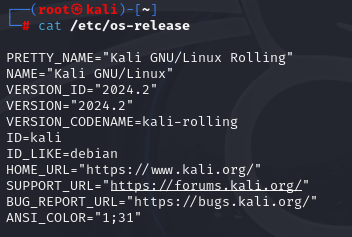
\includegraphics[width=0.6\linewidth]{img2/Imagen1.png} % This is setting the figure to be .75x the width of the line. This can go all the way from 0.1 to 1 (and beyond, but then you're outside the page).
    \label{figura1}
\end{figure}

\subsection{Herramientas} 
Las herramientas que utilizaremos en la maquina virtual seran Docker y Git.
\begin{itemize}
\item Docker: Se utilizara docker para crear las imágenes de todo el contenido necesario para el uso de la aplicación atacada y aplicación atacante. Estas imágenes luego se deben iniciar en un contenedor y exponer en puertos.
\item GIT: lo utilizaremos para verificar el control de version del repositorio donde se descargaran los archivos necesarios para las pruebas.
\end{itemize}

El primer paso es verificar si la versión de Kali a utilizar contiene estas herramientas. En caso de no tenerlas se deben instalar en el ambiente de laboratorio.

Se verifica si docker esta instalado por medio del comando \textbf{\texttt{docker --version}}. Este comando verifica la version de docker instalada en el equipo Figura~\ref{fig:figura2}

\begin{figure}[H]
    \centering
    \caption{Captura para verificar si tenemos docker instalado}
    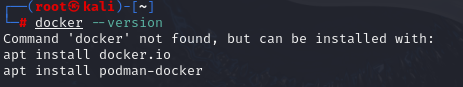
\includegraphics[width=0.6\linewidth]{img2/Imagen2.png}
    \label{fig:figura2}
\end{figure}




\newpage
\section{\large Conclusión}

El rol que hoy juega un Oficial de Protección de Datos es fundamental para las organizaciones que trabajan con datos personales y sensibles, estos datos hoy en día son considerados un activo valioso para las organizaciones las cuales deben y deberán mantener estándares cada vez mas complejos. La importancia de un DPO para algunos estados ya es una obligatoriedad y por ende no solo es suficiente designar una figura para el cumplimiento de este sino es esencial que esta figura tenga las competencias y capacidades para cumplir a cabalidad dicho rol. Esto validara la confianza y la seguridad de sus usuarios.

El DPO dependiendo la organización para la cual desempeñe sus actividades tendrá que poseer conocimientos especializados tanto en derecho, normas y prácticas de protección de datos, así como desarrollar habilidades para la gestión y supervisión del cumplimiento de las normativas vigentes. Debe ser capaz de identificar riesgos para lograr implementar medidas efectivas y fomentar la cultura de la privacidad y sensibilidad de los datos para mitigar la conminación que pueda tener el individuo afectado y garantizar un manejo ético de datos personales.

La figura del DPO es el enlace que debe tener la organización con las autoridades de protección y los individuos cuyos datos son tratados. Su labor aparte de proteger a las organizaciones de posibles sanciones es fortalecer la confianza del usuario y entidades demostrando que es capaz de gestionar sus datos de manera efectiva y responsable.

En conclusión, el papel que juega el DPO es fundamental en el mundo del siglo XXI, ya que asegura que las organizaciones no solo cumplan con las obligaciones legales, sino que también adopten un enfoque dinámico y responsable hacia la protección de datos. A medida que la tecnología y las regulaciones avanzan, la importancia del DPO continuará creciendo, consolidándose como un pilar fundamental en la gestión de la privacidad y la seguridad de la información.


\newpage
% Referencias
\renewcommand\refname{\large\textbf{Referencias}}
\bibliography{bibliography}

\end{document}
